%Edit 0024 ZZZ to report number nnnn 
%Edit 3.1.3 YYMILE to milestone number m.m.m
%Edit Report on user layer design YYTITLE to report title - Words Start with Caps
\documentclass[11pt,twoside,a4paper]{article}
%%======================================================================
%% PACKAGES:
%%
%\usepackage{times}               % Times+Helvetica+Courier fonts
\usepackage{helvet}              % helvetica + cmr
\usepackage{fancyvrb}       % package for headers/footers
\usepackage{amsmath}
\usepackage{amssymb}
\usepackage{graphicx}            % Graphics.
%\usepackage{a4}                  % page layout to fit A4
%\usepackage{lastpage}            % get page no of last page
%\usepackage{ifthen}              % logical branching
\usepackage{hyperref}            %insert hyper-links
\usepackage{latexsym}
\usepackage{verbatim}
%\usepackage{showlabels}
% uncomment the following to override auto page total
%\pptotal{20}
%%======================================================================

% ensure sans-serif font used throughout
\renewcommand{\familydefault}{\sfdefault}

\newcommand{\culhamissueno}{1.00}%<==edit
\newcommand{\culhamshorttitle}{CD/EXCALIBUR-FMS/0024}%<==edit
\newcommand{\Sec}[1]{Section~\ref{sec:#1}}
\newcommand{\Fig}[1]{Figure~\ref{fig:#1}}
\newcommand{\Tab}[1]{Table~\ref{tab:#1}}
\newcommand{\Eq}[1]{Equation~(\ref{eq:#1})}
\newcommand{\Eqs}[2]{Equations(\ref{eq:#1}) and~(\ref{eq:#2})}
\newcommand{\Figs}[2]{Figures~\ref{fig:#1}--~\ref{fig:#2}}
%Bold lc for script names, tt for computer code and file-names
%\F{NEPTUNE} always in caps
\newcommand{\F}[1]{\textsc{#1}}
\newcommand{\B}[1]{\textbf{#1}}
\newcommand{\T}[1]{{\tt #1}}
\newcommand{\V}[1]{\mathbf{#1}}
\newcommand{\I}[1]{\textit{#1}}
\newcommand{\x}{\mathbf{x}}
\newcommand{\bbeta}{\boldsymbol{\beta}}
\newcommand{\pd}[2]{\frac{\partial #1}{\partial #2}}
\newcommand{\fone}{f^{(1)}}
\newcommand{\ftwo}{f^{(2)}}
\newcommand{\fK}{f^{(K)}}
\newcommand{\nep}{\textsc{NEPTUNE}}
\newcommand{\exc}{\textsc{E}x\textsc{CALIBUR}}
\newcommand{\Papp}{Proxyapp}
\newcommand{\papp}{proxyapp}



%%======================================================================

%% REPORT COVER PAGE Information

\newcommand{\culhamtitle}{\LARGE Report on user layer design for
Uncertainty Quantification\\[1.0\baselineskip] M3.1.3 }%<==edit

%%QA BOX information -- change following as needed
\newcommand{\culhamboardname}{Martin O'Brien}%<==edit
\newcommand{\culhamcontactname}{Rob Akers}%<==edit
\newcommand{\culhamauthor}{Wayne Arter}%<==edit
\newcommand{\culhamauthora}{Ed Threlfall}%<==edit
\newcommand{\culhamauthorb}{Joseph Parker}%<==edit
\newcommand{\culhamauthorc}{Debasmita Samaddar}%<==edit
%\newcommand{\culhamcontacttel}{Telephone: 01235 466498}
%\newcommand{\culhamcontactemail}{Email: rob.akers@ukaea.uk}

\newcommand{\culhamdate}{14 October 2020}%<=edit
\newcommand{\culhamdatea}{14 October 2020}%<=edit
\newcommand{\culhamdateb}{14 October 2020}%<=edit

% reproduce Rob's page size

\setlength{\textheight}{220.0mm}
\setlength{\textwidth}{165.0mm}
\setlength{\topmargin}{0.0mm}
\setlength{\oddsidemargin}{0.0mm}
\setlength{\evensidemargin}{\oddsidemargin}
\setlength{\parindent}{0mm}
\addtolength{\parskip}{0.5\baselineskip}
\setlength{\topsep}{0pt}
\setlength{\itemsep}{0pt}

%%======================================================================
\begin{document}

%Titlepage comes out wrong size, but should look right apart from
% picture which cannot be wider than c.150mm.
% To produce conforming report rp1pub.pdf
% remove title page by commenting out lines ending in %<==omit, then
% sed -e '/<==omit$/s/^/%/' < rp1.tex > rp1omit.tex
% pdflatex rp1omit;bibtex rp1omit; pdflatex rp1omit
% pdfunite cover.pdf rp1omit.pdf rp1pub.pdf 
\begin{titlepage}%<==omit
\vspace*{-30mm}%<==omit

\includegraphics[width=2.5cm]{../corpics/cofaplus} \\[2.0\baselineskip]%<==omit
{\LARGE {\textbf{\textsf{ExCALIBUR}}}}\\[2.0\baselineskip]%<==omit
{\LARGE \culhamtitle } \\[2.0\baselineskip]%<==omit
{\textbf{\textsf{Abstract}}}\\%<==omit
The report describes work for \exc \ project \nep \ %<==omit
at Milestone 3.1.3. %<==omit
This report describes techniques of uncertainty quantification~(UQ) that are expected
to prove important for \exc\ project \nep, arranged as they might appear in a
workflow to optimise device design.
First efficient ways of identifying the major sources of uncertainty
are identified, then second, techniques for working with this smaller number are described,
including the production of surrogates.
Third and lastly, UQ analysis is then continued with the
surrogates used to predict distributions of expected outcomes,
with emphasis on producing optimal device designs, which are robust
against say installation errors.\\
%Techniques described under the three headings are respectively\\
%%\begin{enumerate}
%1. Polynomial Chaos Expansion (PCE), Sparse regression (LASSO/Basis Pursuit), Multifidelity Monte-Carlo~(MFMC),
%Multilevel Monte-Carlo~(MLMC)  and Multi-Index Monte-Carlo~(MIMC)\\
%2. Adaptive, sparse quadrature sampling, Forward UQ and Sobol Analysis\\
%3. Surrogate models, Bayesian inference and Optimisation under uncertainty~(OUU)\\
%\end{enumerate}
Since \nep\ software
may be required for a range of applications including comparison with theory,
there is a discussion as to how UQ might best be integrated in the context of \nep, prior to completion
of UQ research work external to UKAEA.


%<==omit
%<==omit
\vfill%<==omit
\centerline{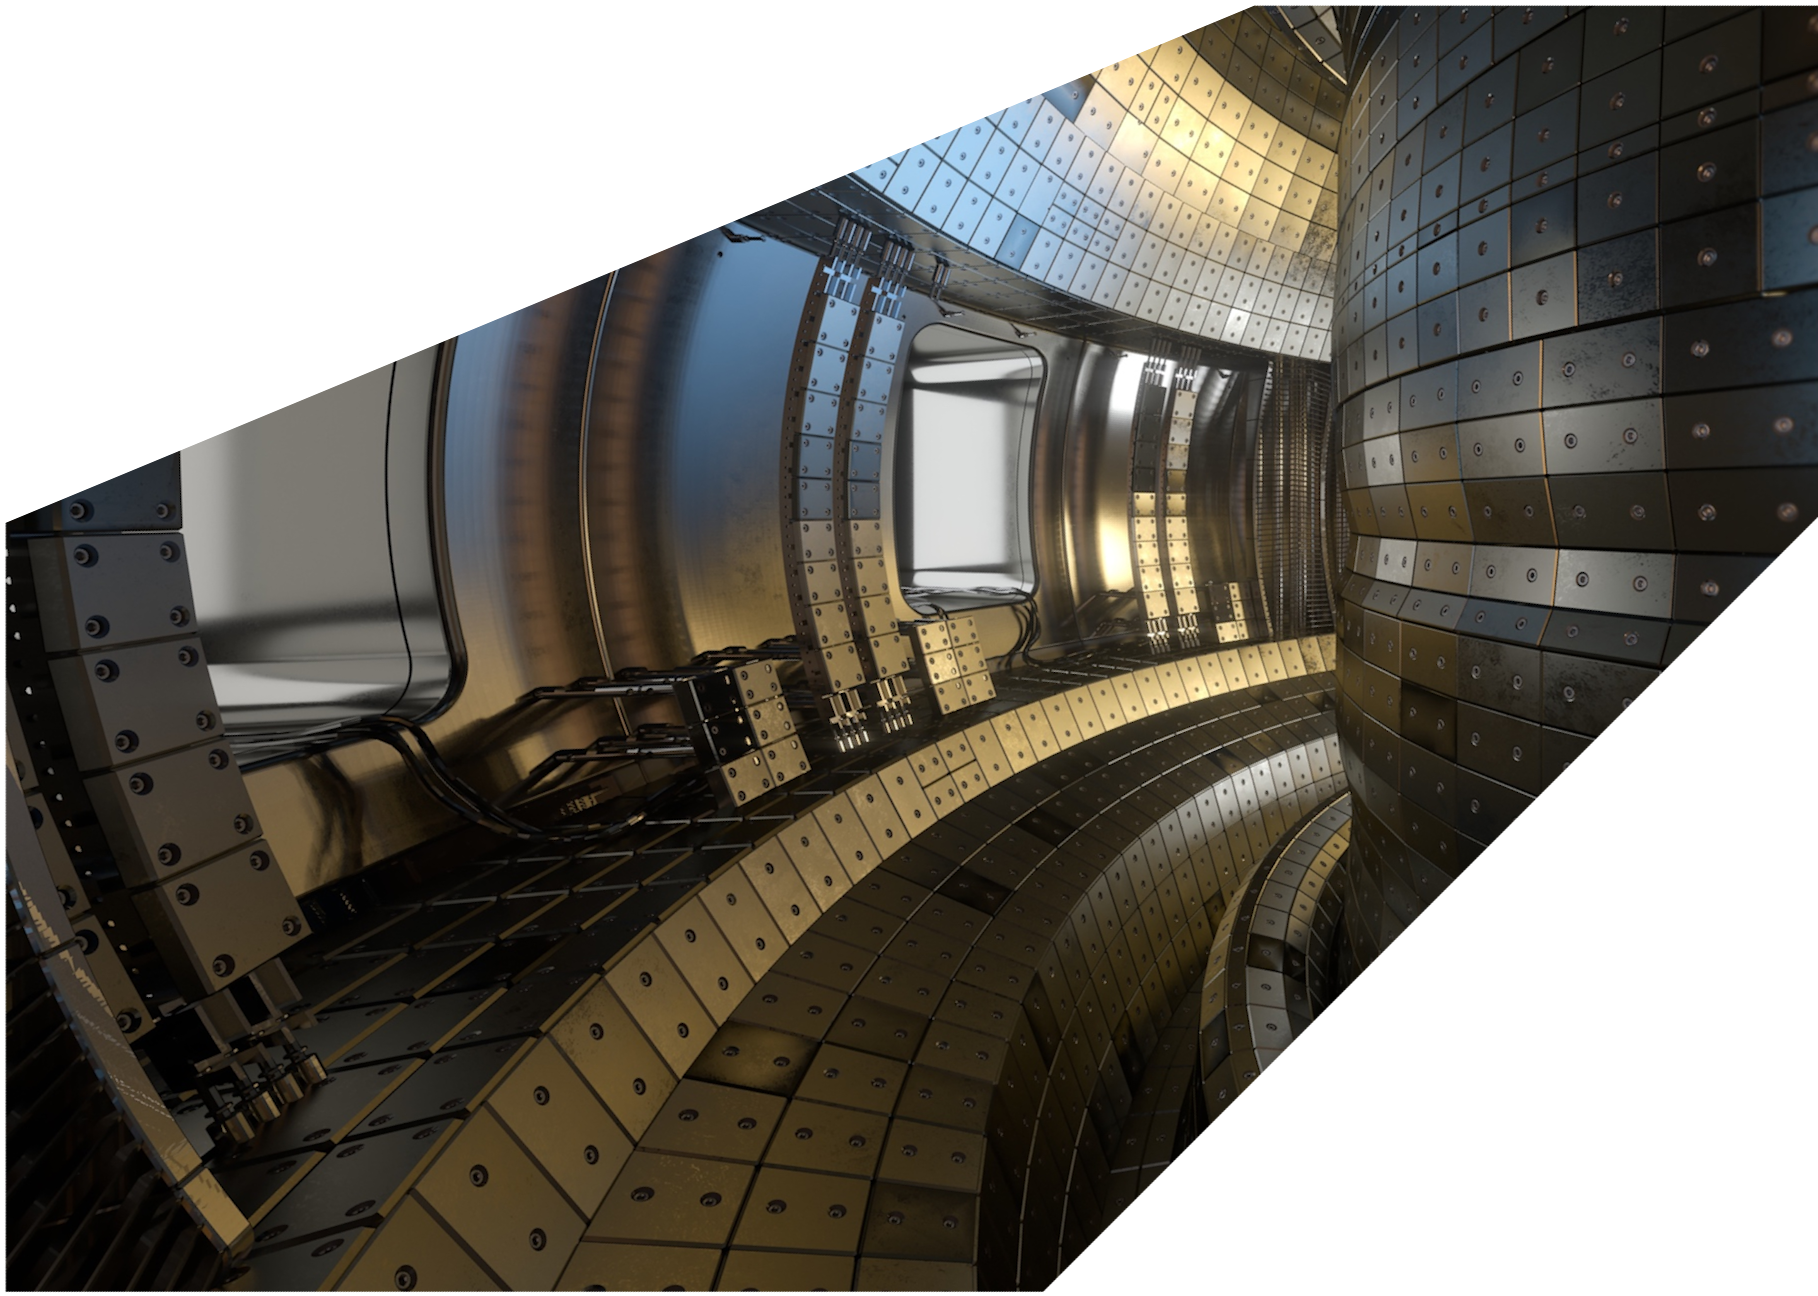
\includegraphics[width=0.9\textwidth]{../corpics/tokintcrop}}%<==omit
\end{titlepage}%<==omit

\hspace{-30mm}\begin{table}[h]
\sffamily
\begin{center}
\textbf{\textsf{UKAEA REFERENCE AND APPROVAL SHEET}}
\begin{tabular}{||p{5.7cm}|p{4.7cm}|p{5.0cm}||}
\hline
\hline
& Client Reference: &  \\
\hline
& UKAEA Reference: & \culhamshorttitle \\
& & \\
\hline
& Issue: & \culhamissueno \\
\hline
& Date: & \culhamdateb \\
\hline
\multicolumn{3}{||l||}{} \\
\multicolumn{3}{||l||}{Project Name: ExCALIBUR Fusion Modelling System} \\
\multicolumn{3}{||l||}{} \\
\hline
\end{tabular}
\begin{tabular}{||p{3.3cm}|p{4.6cm}|p{3.5cm}|p{3.6cm}||}
\hline
& Name and Department & Signature & Date \\
\hline
Prepared By: & \culhamauthor & N/A & \culhamdate \\
& \culhamauthora & N/A & \culhamdate \\
& \culhamauthorb  & N/A & \culhamdate \\
& & & \\
& BD & & \\
\hline
Reviewed By: & \culhamcontactname & 
\includegraphics[width=3.0cm]{../corpics/blanksign}& \culhamdatea \\
& & & \\
& Advanced Computing Dept. Manager & & \\
\hline
Approved By: & \culhamboardname  & 
\includegraphics[width=3.0cm]{../corpics/blanksign} & \culhamdateb \\
& & & \\
& MSSC & &\\
\hline
\hline
\end{tabular}
\end{center}
\end{table}


\clearpage
\section{Introduction}\label{sec:intro}
This report has the goal of consolidating earlier work regarding software
design patterns \cite{y2re332} by attempting an initial identification of
specific patterns to be applied in the forthcoming \nep\ \papp s, and also
summarizing some other general design concerns.

Section \ref{sec:proxypat} identifies patterns relevant to
specific core \nep\ \papp s.
It is noted that two of these \papp s are to be based on pre-existing
object-oriented (C++) frameworks and the task is made easier by the explicit
identification of some of the relevant patterns in those frameworks'
accompanying documentation.
Those are the \papp s that are to treat continuous fields; an additional part
describes one of the \papp s designed to treat particles, which at the time 
of writing is intended to be based on a procedural code written in Fortran.  
Further insight into the use of design patterns in Fortran, and more generally the
construction of complex modular frameworks, can be 
gleaned from the study of existing codes; to this purpose, a discussion of 
the \F{SMARDDA} simulation framework is included.
Following sketches of the \papp s, a shortlist of relevant design patterns is
given.

Section \ref{sec:overarchpat} presents some overarching concerns
relevant to the initial \papp\ ecosystem as a whole, viewed here as a
fledgling multiphysics ecosystem and keeping in sight the likely structure of
exascale target hardware.
The first annex \ref{sec:gamestruct} demonstrates one tangentially relevant approach
to handling a complex software ecosystem.
As in earlier work, a general dearth of published material treating patterns in
scientific programming is noted, indicating that room is left for more definite
strategies for the overall \nep \ framework, once the initial implementations
of the \papp s become available.

A second  annex \ref{sec:proxyapp_standards} contains a precis of a set of standards
for scientific \papp s and a framework for benchmarking the same proposed by
the US Department of Energy's Exascale Computing Project.

\clearpage
\section{Design patterns for individual \nep\ \papp s}\label{sec:proxypat}

In this section, descriptions of the \papp s that will be created under three of
the project \nep\ calls are given:
in subsection \ref{sec:call1} the \papp\  for Call 1, ``Examining the
performance of Nektar++ for fusion applications'',
in subsection \ref{sec:call6} the \papp s for Call 6, ``Fluid referent models''
and in subsection \ref{sec:call8} the \papp s for Call 8, ``Development of a
gyro-averaged referent model''.
A further subsection \ref{sec:smagain} contains a discussion of the existing 
\F{SMARDDA} modules framework.
Finally, in subsection \ref{sec:design_pattern_individual_\papp s}, a discussion
of the different design patterns employed in the \papp s is provided.

\subsection{Software design patterns for Call 1 Proxyapp}\label{sec:call1}

%Description of proxyapp

The proxyapp specified in Section 2.1.5 of Contract Ref.\ T/NA078/20, {\it Proxyapp instantiating a 2D model of anisotropic heat transport}, is designed to investigate and quantify the performance of spectral element methods \cite{karniadakissherwin} in modelling anisotropic heat transport in close proximity to a complex first wall geometry.
The initial remit is for a two-dimensional solver only.
It is worth noting that a rather generic requirement for next-generation algorithms is spectral accuracy, not least because it is suited to the current HPC landscape - hence, some of the design patterns used in this proxyapp are expected to bleed into other \nep\ work.

%Context of proxyapp

The proxyapp will be built within the pre-existing {\it Nektar++} framework for spectral / hp element PDE solvers \cite{nektarwebsite} and will extend current capabilities to include equations governing the scrape-off layer plasma.  
The higher-order methods used by {\it Nektar++} generically involve a large amount of arithmetic for a given quantity of data, a computational pattern that is well-suited to today's HPC landscape.  
The scope of the problem encompasses also techniques for generating two- and three-dimensional meshes capable of conforming to a reactor wall and also to the geometry of local magnetic field lines representing, for example, the tokamak X-point and this capability will be provided by {\it NekMesh}, a meshing framework capable of importing computational meshes from popular CAD formats as well as generating its own meshes and which is integrated with {\it Nektar++} \cite{nektarwebsite}.

%Patterns with UML diagrams

The proxyapp has yet to be implemented but in view of the facts that it will leverage existing {\it Nektar++} code and that codes of this type are likely to have certain common and well-defined characteristics, a description of the main software design patterns used in the {\it Nektar++} framework is presented (for more details, see the discussion in Section 3.5 of \cite{nektardevelopersguide}).


\subsection{Software design patterns for Call 6 Proxyapps}\label{sec:call6}

%Description of proxyapps

The Contract Ref.\ T/NA083/20 specifies the creation of five proxyapps to
mirror the development of the referent fluid model.
This model will capture the physics in the tokamak edge, including the
separatrix but away from the core and from the metal surfaces of the device.
It is to include the multi-physics phenomena relevant to the tokamak exhaust
(bulk plasma species, impurities and neutrals).  
The code itself must be performant and scalable to Exascale, easy to deploy
upon different architectures, and actionable (i.e.\ include treatment of
uncertainty quantification, UQ).  
Moreover it must couple efficiently to the neutral gas and impurity model, and
the 5D gyro-averaged model developed in other work packages.

The five proxyapps are largely independent, focussing on separate aspects, namely:
\begin{enumerate}
	\item 2D elliptic solver in complex geometry
	\item 1D simplified fluid model with UQ and realistic boundary conditions
	\item 1D model incorporating velocity space effects
	\item 1D multispecies plasma model
	\item 2D model incorporating velocity space effects
\end{enumerate}

%Context of proxyapp

The two proxyapps focussing on velocity space effects (proxyapps 3 and 5) will draw on work on
kinetic solvers, and will be written in a high-level language such as Python or Julia.
For each of the remaining proxyapps, two versions will be developed for
comparison, one in BOUT++ \cite{BOUT++} and one in Nektar++.
As mentioned above, Nektar++ is a framework for solving PDEs with spectral/hp, which will be extended as part of Call 1 to include terms relevant for plasma physics.
In contrast, BOUT++ is a framework for solving plasma and fluid-like equations in curvilinear coordinates using finite-difference approaches,
but lacks the complex meshing and finite element approaches of Nektar++.

Proxyapps 2 and 4 above investigate the feasibility of including new physics
(namely realistic sheath boundary conditions and multiple species). 
For this, new terms will be added to the existing BOUT++ physics modules, SD1D
and Hermes-3.
Owing to BOUT++'s domain specific language, these additions will be relatively
straightforward (from a software development perspective).

The remaining proxyapp (number 1) will be implemented by coupling BOUT++ to
elliptic solvers provided by PETSc and Hypre.
BOUT++ uses the strategy pattern (see section \ref{sec:strategy} below) to implement different elliptic solvers.
BOUT++ also makes use of the template method (section \ref{sec:template}) and abstract factories (section \ref{sec:abstract_factory}).


\subsection{Software design patterns for Call 8 Proxyapps}\label{sec:call8}

%Description of proxyapps

The Contract Ref.\ T/NA085/20 focusses on the development of a referent
gyrokinetics model.
This work package will investigate a novel approach to deriving the gyrokinetic
equations, where the local three-dimensional fluid quantities (density,
momentum and energy) are embedded into the five-dimensional particle
distribution function.
This leads to a version of gyrokinetics with both a kinetic equation for the
modified distribution function and a set of fluid equations for the local
moments.
This allows one to use a single model to study both the core (where one solves
the whole equation system) and for the scrape-off layer (where one solves 
only the fluid equations).
Alternatively, the model allows a very natural coupling of the gyrokinetic
equations to any set of fluid equations for the scrape-off layer.

Because of the novelty of this approach, the work package will first derive
drift kinetic equations (the simplified, long-perpendicular wavelength
limit of gyrokinetics).
It will also develop proxyapps to compare the numerical performance of the new
model to a more standard drift kinetic model for a variety of problems.
It will determine potential bottlenecks in the numerical treatment of the drift
kinetic models, and, in addition, develop appropriate numerical algorithms for
treating the wall boundary.

%Context of proxyapp

The proxyapp will be developed from scratch using Julia, which combines rapid
prototyping in a high-level language and access to computational libraries,
with performance that approaches that of statically-typed languages. 
While there is no design pattern yet specified for the proxyapp, the developers
are also early contributors to the gyrokinetics code GS2 \cite{GS2}.
It therefore seems likely that the proxyapp will share design features with
GS2.

GS2 is written in Fortran 90, using a modular design pattern (see section
\ref{sec:modular}).
It utilizes lazy initialization (see section \ref{sec:lazy_init}) as a
technique to passively manage module dependencies.
The modular design is a result of the age of the code.
Object-oriented techniques have been introduced, but in an incremental
fashion that allows modular design to coexist with encapsulated objects.
To achieve this, dependency injection (section \ref{sec:dependency_injection})
was adopted, with module-level variables being phased out in favour of large
\texttt{state} objects.
Having a small number of objects with many members has proven convenient for developers,
and it seems likely this proxyapp will retain this approach from GS2,
with perhaps a few \texttt{state} objects representing the solution, the diagnostic outputs
and the simulation parameters.

%%%GS2 is written in Fortran 90, using a modular design pattern.
%%%It utilizes lazy initialization -- rather than handling dependencies between modules explicitly,
%%%each module has an initialization subroutine \texttt{init} which calls the \texttt{init} routine of all the module's dependencies before initializing itself.
%%%A similar approach is taken to uninitialization.
%%%In keeping with the modular design, GS2 makes heavy use of module-level
%%%variables for objects like the solution arrays and grid resolutions.
%%%These variables may be read and modified by all subroutines within the module;
%%%when given the \texttt{public} attribute, such variables may be edited by \emph{all} modules.
%%%The module-level variables arise in legacy code, and the newer code
%%%incorporates object-oriented designs.  
%%%However, this change was made incrementally, with the object-oriented code
%%%coexisting with the module-level variables.
%%%Therefore, the object-oriented approach uses a dependency injection design pattern, 
%%%where so far as possible, objects that were previous module-level variables
%%%are instead wrapped into a large \texttt{state} object.
%%%The \texttt{state} is then the input/output of subroutines, allowing the
%%%module-level variables to be incrementally removed.
%%%Having a small number of objects with many members has proven convenient for developers,
%%%and it seems likely this proxyapp will retain this approach from GS2,
%%%with perhaps a few \texttt{state} objects representing the solution, the diagnostic outputs
%%%and the simulation parameters.

\subsection{\F{SMARDDA} modules framework revisited}\label{sec:smagain}
The \F{SMARDDA} modules framework was discussed briefly in the M3.1.2 report~\cite{y2re312},
where particularly its layered structure was noted as relevant to \nep.
Exploration of the literature since, as described in the earlier
\Sec{call1}--\Sec{call8}, has indicated that it is both common and commended
by many workers to construct complex software through aggregation of smaller objects
that may themselves be the basis for physically separate codes. Since the
\F{SMARDDA} software is also built using aggregation in this way, a more
detailed description of this is provided here.

As previously mentioned~\cite{y2re312}, the \F{SMARDDA} software is coded in a
Fortran language style documented in a Culham report~\cite{fprog}
(which is in fact very similar to other styles recommended in the meteorological
community) exemplified by templates which have been posted on github,
as program smardda-qprog~\cite{qprogwebsite}. The new material presented here treats \I{qprog}
as a standalone, independent of the \F{SMARDDA} modules, to emphasise its structure.
Note that the name `qprog' has been deliberately chosen so as not conflict
with other software, the `q' indicating that it poses all the questions to the
developer, since it is purely a skeleton framework accepting nominal inputs
to produce nominal outputs.

Layering is represented by the presence of a
subdirectory LIB, containing a subroutine library compiled from Fortran 
conforming to the older \F{FORTRAN-77} standard. In practice if not in implementation,
the Fortran~95 utility routines which duplicate many of the functions of the
old OLYMPUS library~\cite{y2re312} also share this layer. The most widely used
of these utilities  is log\_m for logging progress made by the code including errors,
and timing information for which modules date\_time\_m and clock\_m are also needed.

There is a script qprog.bash in the repo~\cite{qprogwebsite}
which will set up the files, see \Tab{qprogfiles}, making up a conforming program, and indeed
try to compile, link and run it.
(It does not need \F{SMARDDA} installation if -l for locally complete is set as the first option.)
It is perhaps easiest to start understanding the framework from the documentation of the script.
The program name, its abbreviation (typically one or two letters) and description are defined using
the keys QPROG, Q and STR. The name of a skeleton object module to be tested, its abbreviation
and description are defined using the keys BIGOBJ, BO and BSTR:
\begin{verbatim}
qprog.bash [-l] \
QPROG=xpc Q=xp STR="transport_coefficients" \
BIGOBJ=clcoef BO=cc BSTR="classical_coefficients"
\end{verbatim}
The example is that of a code \I{xpc} to calculate transport coefficients, where
the program name also corresponds to an object, which in this case is the set of
transport models. In the example, for simplicity's sake, only one physical model,
giving the so-called classical or Braginskii coefficients is considered, as object clcoef.
The relation between the objects is shown in \Fig{xpch}. In the example, all objects
are `big', ie. the object description is separated in a file with name ending ``\_h"
from the subroutines which operate on the object in a file with name ending ``\_m",
thus clcoef\_h and clcoef\_m. For a small object, object and associated subroutines
are both combined in one module (``\_m") file. Whereas the full name is used to
describe the namelist QPROGparameters associated with the object 
(namelist is a Fortran language feature for user-friendly keyed
input of values for code variables),
the abbreviation is used to produce type names associated with the object,
notably type Qnumerics (or BOnumerics, xpnumerics and ccnumerics
respectively in the example). The latter separates out the data needed to define
the object, making it possible for instantiation to be deferred (`lazy initialisation').
There is also produced a control module xpcontrol\_m for the program object.

As the templates indicate, each object is largely self-contained within its
module, with subroutines for opening a file which contains input control data, reading from it
and closing it, together with output routines. These latter routines manage files which
might contain numeric dumps of the object variables and descriptions of the
object in plotting formats defined for {\it gnuplot} and {\it ParaView}, to be used in post-processing 
and to visualise aspects of the object in up to 3-D.

The calling tree shown in \Fig{xpc} indicates how the calls, starting with {\tt xpcontrol\_read}
(note the use of the abbreviation in the subroutine name), are arranged so that input data
defining all the objects can be read from a single file.
The $1, 2, 3$ layout is used by the main program xpc~\cite{y2re312}
where in sequence order, $1$~is initialisation, $2$~is compute and $3$~is output and closedown,
but this layout is not generally suitable for use by the other objects.

It is worth noting that there is a .log file
with a special status designed to ensure that as far as possible diagnostics are captured
even should serious errors occur.

It will be seen that, assuming the coefficients of the various transport models combine to
give the total transport by the plasma,  the code will in essence implement the puppeteer
pattern despite the constraint
of a single control file, in that the clcoef\_m  module (and consequently other modules
that might be written to define other sets of coefficients) knows nothing about the \I{xpc} object.
Information needed by clcoef and sibling modules, such as details of the plasma composition, is to be passed
to them in module xpcontrol\_m. The present implementation of this last in xpcontrol\_m
is inelegant, and only adequate for a simple example. For more realistic applications,
understanding and mapping the dependencies between the various inputs will likely
require a graph-based elaboration on the present code design.

Extension to other sibling models such as anomalous transport should be straightforward.
All that has to be arranged is for {\tt xpcontrol\_read} to call {\tt anomcoeff\_readcon},
{\tt xpc\_solve} to call {\tt anomcoeff\_solve} and the various output routines {\tt xpc\_writev},
{\tt xpc\_writeg} and  {\tt xpc\_write} to call their equivalents in the transport coefficient objects.

It is also worth mentioning that use of templates enabled the production of over $1\,400$~lines
of potentially tricky code logic from about $50$~lines of pseudo-code defining variables to be found
in the repo files qprog.txt and clcoef.txt plus
the $2$~lines defining QPROG, Q, etc. above, using a
lengthy but relatively straightforward script, and the total line count allowing
for the utilities is nearly~$4\,000$. In fact the bulk of the remaining code to evaluate classical
transport coefficients to be found on the web-site~\cite{miscwebsite}  was produced with
the help of the reduce-algebra
package~\cite{reducewebsite} which can output mathematical expression in a Fortran syntax.

\begin{table}[h]
\begin{center}
\caption{Files and principal input functions of the QPROG code (xpc example).
The .f90 suffix has been omitted from the filenames.
\label{tab:qprogfiles}}
\begin{tabular}{|p{2.5cm}|p{12.5cm}|}
\hline
File &  Description \\
\hline
QPROG & main program, see its sequence diagram in \Fig{xpc} \\
QPROG\_h & parameters collected in type Qnumerics\_t describing how to construct (at least one) object BIGOBJ
 which is to  be combined with other object data structures such as BIGOBJ\_t into type QPROG\_t \\
QPROG\_m & calls {\tt QPROG\_readcon}, which reads namelist variables 
listed in QPROGparameters and copies them to type Qnumerics\_t variables \\
Qcontrol\_h & data structure of generic top level controls for QPROG (abbreviated as Q) \\
Qcontrol\_m & object of generic top level controls for QPROG (abbreviated as Q), calls {\tt BIGOBJ\_readcon}
 via {\tt Qcontrol\_read} \\
BIGOBJ\_h & data structure of controls for BIGOBJ forming type BOnumerics\_t, also combined type BIGOBJ\_t \\
BIGOBJ\_m & object which reads in object level controls\\
\hline
\end{tabular}
\end{center}
\end{table}


\begin{figure}
\centerline{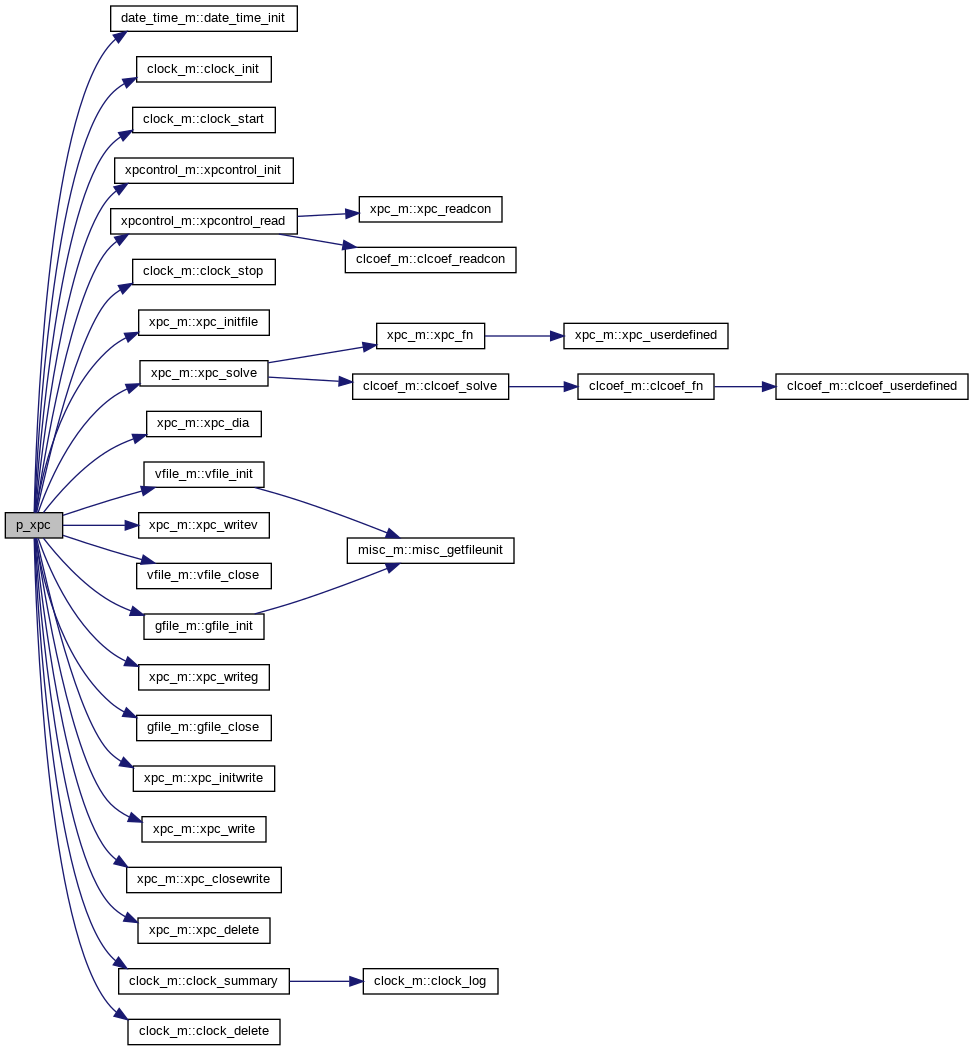
\includegraphics[width=12cm]{../pics/xpc}}
\caption{Calling structure for \F{SMARDDA} style program, plot produced by doxygen
which in this example largely imitates a UML sequence diagram.
The important subroutines to note are {\tt xpcontrol\_read} which coordinates the input of data
defining the two objects clcoef\_t and xpc\_t, and {\tt xpc\_solve} which calls subroutines
operating on both objects to do the work of the code.
(Calls to log\_m subroutines have been suppressed for clarity.)
\label{fig:xpc}}
\end{figure}
\begin{figure}
\centerline{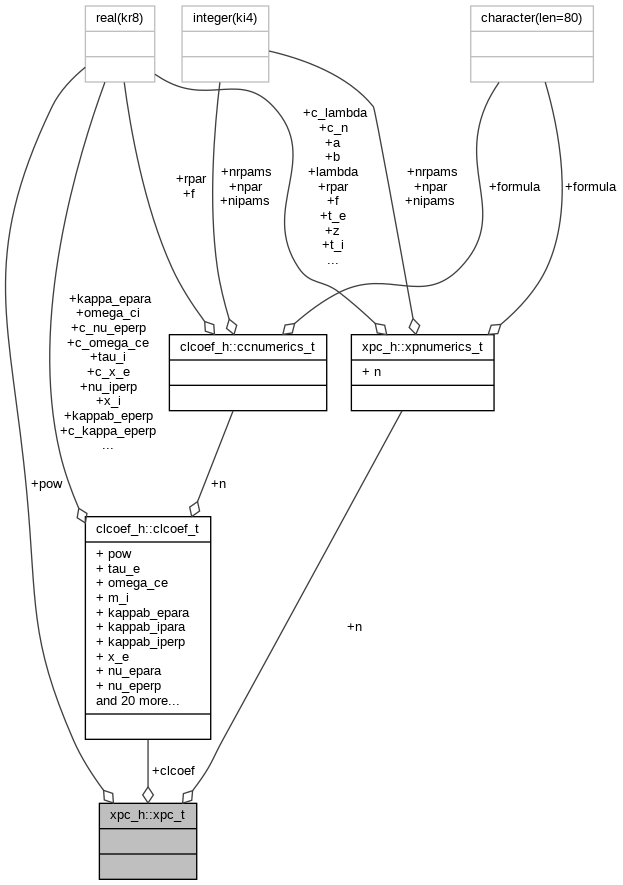
\includegraphics[width=12cm]{../pics/xpch}}
\caption{Data structure for \F{SMARDDA} style program. The plot produced by doxygen
unhelpfully links variables to their simple types (real, integer and character),
however it should be clear each object is associated with a numerics type that
defines how it is to be generated. The figure also indicates how objects are aggregated,
in this instance there is only one object clcoef\_t aggregated with the code level
controls to form the code object xpc\_t.
\label{fig:xpch}}
\end{figure}

\clearpage
%\subsection{DSL-like feature}
%Files input
%qprog.txt contains the input variables that might be used by a range of different objects/modules
%and the default values for these inputs. These variables form part of the top level control QPROG_t
%for the program. A human readable variable for use in
%a namelist will be generated using the first 3 words of the description of each variable.
%In the example, a=... to lambda=... will be copied to QPROG.txt (xpc.txt) and finish in QPROG_h.f90
%bigobj.txt contains the variables defining one object which will normally be defined using the
%instructions resulting from the input variables in qprog.txt, using additional object level controls
%(and of course code to be written by the user).
%In the example, tau_e... and c_tau_e... will be copied to BIGOBJ.txt (clcoef.txt)
%and finish in BIGOBJ_h.f90.
%makefile.QPROG makefile to compile and link QPROG 
%QPROG\_case0.ctl & input file for QPROG containing complete list of namelists
%
%Outputs from execution of QPROG
%xpc\_case0.log log data such as date and time of run, cpu measured by internal clocks
%xpc\_case0\_xpc.out indicative output, precisely object level controls for BIGOBJ

\input{design_patterns_neptune_\papp s}
\clearpage
\section{Overarching design patterns for \nep}\label{sec:overarchpat}

\subsection{Domain-specific patterns for scientific computing}

This section reflects the state of \nep\ at the time of writing: there are, as
yet, no detailed designs for the proxyapps (this is the division between
specification and development); and as a result, this report is correctly to
be regarded as a living document.
That said, some progress can be made by realizing that the forthcoming
proxyapps form the prototype components for a modular scientific simulation
framework fitting precisely the description of a {\it System for modeling and
simulation} given by Sommerville~\cite{sommerville}:

\begin{quote}
These are systems that are developed by
scientists and engineers to model physical processes or situations, which include
many separate, interacting objects. These are often computationally intensive
and require high-performance parallel systems for execution.
\end{quote}

It is for example clear at this point that the lion's share of the \nep\ code
will be written in object-oriented languages: most of the core proxyapps will
be written in C++ in order to leverage existing componentized frameworks (as
mentioned above, the {\it Nektar++} framework makes extensive use of
object-oriented methods~\cite{Mo20Nekt}).
Accordingly, much of the tried and tested pattern language developed in
\cite{gammahelmjohnsonvlissides} and thereafter is relevant (and, further,
the proxyapps have the potential to benefit from the advantages of the Object
pattern described by Rouson et al in Ch.5 of~\cite{rousonxiaxu}).  
As regards the trade-off between object-oriented coding and ultimate
performance, it might be noted that these frameworks have proven scaling to
at least thousands of processor cores.

Applications of software patterns to scientific computing are yet more
directly germane, if sadly rare: the current edition of \cite{rousonxiaxu}, a
textbook aiming to provide a lexicon of domain-specific design patterns aimed
at multiphysics applications, was published in 2014 and it explicitly
highlights (p.6) the relative paucity of references for design patterns
specific to scientific computing as of that date.
The book culminates in the Morfeus framework, a proposal that seems to have
been aimed at providing an implementation of many of the book's ideas, though
it restricts itself to Fortran.
Some other salient domain-specific patterns are outlined in the article by
Blilie \cite{Bl02Patt}, including, for example, how to handle quantities
with physical units.
Quantities with units raise a number of concerns in scientific programming: a
judicious choice can result in simplification of the code, eliminating
unnecessary floating-point operations (one straightforward example is
removing $\epsilon_0$ and $\mu_0$ when simulating Maxwell's equations, by
rescaling the variables representing the magnetic field and the time), as
well as improving readability; and a consistent overall strategy for units is
obviously required when coupling different proxyapps.
This paper highlights also the fact that design patterns can help in the
division of labour between domain specialists (i.e. physicists) and experienced
software engineers, in that those specialists can use the UML representations
to specify the code structure in a language-independent form, to be
implemented in detail by software developers with little or no domain
expertise.
In addition, \cite{Bl02Patt} outlines two general patterns to be used for
treating the generic types of problem treated by physics software: particles
on one hand and continuous systems (a.k.a fields) on the other, highlighting
that useful simplifications can be made in order to handle multiple timescales
(for example, updating the fast particle dynamics at a higher time resolution
than that of the fields), though a note of caution is sounded if the physics
of the problem is tightly coupled.

\subsection{Architectural patterns}

Architectural design patterns occupy a level just beneath that of the overall
application framework (into which falls the question of division into
libraries and appropriate directory structures) and were first defined by
Garlan and Shaw in 1996 \cite{garlanshaw}, there called {\it architectural
styles}.  
They govern overall program control and coordination.  Given the incremental
development and delivery strategy adopted in \nep, a detailed discussion of
the final architecture (falling under the definition of {\it architecture in
the large} given in ch.6 of Sommerville \cite{sommerville}) is perhaps
premature at this point.  
In future, wisdom in this area could be gleaned by closer study of existing
architectures, for example the United States' {\it One Modeling Framework for
Integrated Tasks} (OMFIT) system \cite{omfitwebsite} and the ITER {\it
Integrated Modelling and Analysis Suite} (IMAS) \cite{Im15Desi}, the latter of
which uses the Kepler scientific workflow system \cite{keplerwebsite}, even
for fine-grained component integration.  
On an individual proxyapp level, called {\it architecture in the small},
application architectures are again determined to an extent by the re-use of
existing frameworks.

One interesting scheme is the layered architectural pattern, which, as well as
giving localization of change, may be used to provide performance portability;
as a topical example, algorithmic content could be implemented in terms of the
API of an abstraction layer such as SYCL \cite{syclwebsite}, Kokkos
\cite{kokkoswebsite} or RAJA \cite{rajawebsite}.  
Although there is a one-off overhead in writing the initial implementation in
terms of the chosen API (though some aim to provide a C++-like programming
experience), the code is thereafter portable between any of the platforms supported
by the abstraction layer, with little additional programmer burden (see
Fig.\ref{fig:sycllayer}).  
These abstraction layers are somewhat new technology at the time of writing
and it is certainly possible to envisage cases in which the performance achieved might
be bettered by a platform-specific implementation (though see
\cite{De20Eval} for an analysis of the relative performance of
SYCL vs. native code for a standard benchmark based on HPC-style
applications).  
This paradigm offers a potential route to a more sustainable code, since the
abstraction layers avoid tying to one platform; moreover, they may also be
extensible to future accelerator types.  
It is also a significant step in the direction of what Rouson et al
\cite{rousonxiaxu} refer to as the holy grail of parallel scalability, to wit
{\it automatic parallelization of code without direct programmer
intervention}.

\begin{figure}
\centerline{\rotatebox{0}{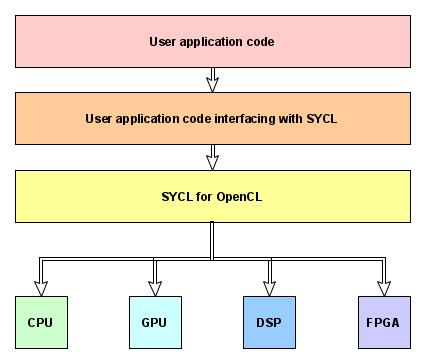
\includegraphics[width=10.5cm]{../png/sycl_layer.jpg}}}
\caption{\label{fig:sycllayer}
Diagram illustrating layered structure of an application using an abstraction layer (SYCL here).  Only the layer directly addressing SYCL would require recompilation to port the code between different accelerator types.}
\end{figure}
\clearpage
\subsection{Concurrency patterns for the exascale}

Although at a hardware level, the current HPC scene is something of a
menagerie, the schema common to all conventional modern systems is that of a
large array of individual compute units (themselves subject to the further
comminution of varying degrees of vectorization), a structure that mandates the
parallelization of algorithms in order to obtain good performance.  
Indeed, running on such a machine, any subsection of a code that cannot be
efficiently parallelized ultimately becomes a performance bottleneck (Amdahl's
law).  
This leads to a selection of concurrency design patterns aimed at the
production of efficient parallel code \cite{softwarepatternwiki}: the main
goal (alongside certain admittedly critical housekeeping duties) is to
preserve strong scaling (assuming that good node-level performance has been
achieved) thus making sure that the supercomputer is not functioning as less
than the sum of its parts.

One key pattern is that of a Compute Kernel: a routine compiled for use on a
high-throughput accelerator.  
This idea has its origins in the pixel shader units of GPUs and typically
applies the inner loops of algorithms, being geared toward vectorized
processors and SIMD by virtue of its repetitious nature.  
One concrete example to be incorporated in \nep\ spectral / hp element
proxyapps is an optimized Compute Kernel for the anisotropic Laplacian
operating on fields in a finite-element expansion basis.  
Following an initial baseline implementation on sequential x86, optimized
versions targeting x86 vector intrinsics, NVidia and Arm are anticipated. 
The efficiencies here are furthered by exploiting the sum-factorization of
fairly sparse matrices that is possible for certain classes of finite
elements.  
Thus, the Compute Kernel pattern is expected to play a key part in obtaining
good performance for \nep\ proxyapps, though there is a little tension between
this plan -- interchangeable, machine-specific kernels -- and the more
visionary abstraction layer philosophy described in the preceding section.

Patterns also exist for parallel I/O: the current version of {\it Nektar++}
uses parallel-friendly mesh input files (in order to avoid the bottleneck of
an individual processor parsing single-handedly a large mesh) and data
checkpoint files. Mesh data is now stored in HDF5 format rather than XML; and
in reading a mesh, a domain decomposition is performed, using the PT-Scotch
library~\cite{Mo20Nekt, scotchwebsite}.

Future exascale systems following the current pattern of large numbers of
compute units are expected to mandate patterns for fault tolerance and error
handling: see, for example, the discussion of resilience engineering in
\cite{sommerville}.  This will be of particular importance for any code
involved in the control of a fusion reactor.

\subsection{Coupling patterns}

It will be necessary to couple the physics represented by initially separate proxyapps.  
One goal of Contract Ref. T/NA078/20 is to provide proof-of-principle coupling between
the proxyapp and another compatible solver, using the coupling framework that
already exists, and has been proven, within the {\it Nektar++} framework.
This works by providing point-located field values and their respective
locations via the MPI-based CWIPI framework~\cite{cwipiwebsite,Ca19Test}.  
There are a number of issues here, including the computational overheads of
such a scheme, and the need to convert data formats - even between two solvers
using spectral / hp elements methods, there is still a large amount of choice
among this family of methods and the optimal choice for one application is
unlikely to match precisely with that of another.  
It is also critical that spectral accuracy can be preserved during such a
conversion (this would boil down to ensuring that the data sampling is of
sufficient density to avoid aliasing, cf. the number of sample points needed
to perform Gaussian quadrature of polynomials of a given order).  
More generally, compatibility of the data passed between different proxyapps
could be assured by using the Gang of Four Adapter design pattern to provide a
translation between any differing data requirements.  
In the context of the IMAS framework mentioned above, a specific example of an Adapter
is provided by OMAS (Ordered Multidimensional Array Structures) \cite{omaswebsite}, 
a Python library used to interface IMAS to other codes.
OMAS implements a replica of the data structures used in IMAS, supports other popular
file formats (e.g. NetCDF and HDF5) and also is capable of automatic coordinate 
convention transformations, grid interpolation, units conversions, and the calculation
of physics quantities of interest from the fundamental variables.
An additional issue for \nep\ is the need to couple outputs to AI / surrogate generators
in future and, as these may operate at reduced numerical precision, a coupling
framework capable of variable precision would seem to be indicated.


The Puppeteer pattern described in \cite{rousonxiaxu} provides a means of
coupling multiple abstractions in a way that a) is efficient in terms of the
number of couplings and b) uses only the public interfaces of individual
modules and is thus a candidate for implementing a coupled multi-physics
framework.  
The existence of this pattern provides a potential strategy for the future
coupling of proxyapps into a true multiphysics framework capable of handling a
potentially large number of individual physics components, for example fluid
and kinetic models, particle dynamics and atomic physics.

\clearpage

\clearpage
\section{Summary}\label{sec:summ}
This report has arranged the statistical and applied mathematical techniques of UQ 
according to a likely \nep\ workflow for device optimisation.
Other workflows have been considered, see \Sec{impl} where a need is
recorded to treat code validation against theoretical models 
including comparison with experiment.

Other authors arrange the subject of UQ rather differently,
thus the textbook of Smith~\cite{smithUQ} treats additional topics under the headings
of ``Model Calibration" and ``Parameter Selection", which loosely correspond to Stages 1~and~2
respectively, ``Uncertainty Propagation" which corresponds to Stage~2
and ``Model Discrepancy" which corresponds to Stage~3.
Regarding the COSSAN software~\cite{Pa14Open}, there is a toolbox arrangement.
Thus sampling (grouped with interval/subset methods under the heading of ``Reliability"),
meta-modelling, sensitivity and optimisation are treated under separate headings.
Under each heading there is found a range of possible tools or methods, partly to provide a check,
but also because newer methods may be worth exploration, or 
because the best method may be problem dependent.
For instance, for sparse system identification, SLSQT (see \Sec{sparsereg})
proved very successful for Brunton~et~al~\cite{Br16Disc}, but selecting an
appropriate threshold value for SLSQT may not as easy in other applications.
Each software tool may employed in different combinations with the others at different stages,
eg.\ optimisation may be used both in Stage~2, to fit surrogate models better, and in Stage~3
in conjunction with sampling to treat uncertainty, to improve a design.

The nub of UQ is finding an affordable, good surrogate for the full model.
The applicability of a lower-dimensional surrogate model 
often results from the fact that a physical system, in normal operation, behaves `smoothly'
ie.\  the sensitivity of its output function to changes in input parameters is rather low. 
The work of Trefethen~\cite{To15Cont,Ha17Cheb,Tr20Priz} indicates that
approximately~$80$\,\% of functions encountered in practice (most
likely meaning related to use of the matlab$^{TM}$ software) may be
efficiently and accurately approximated as sums of products of functions
of a single variable, suggesting they are representable by say, of order~$100$-$1000d$ samples
if there are $d$~parameters.
%However, it is not necessarily obvious which functions fall into the awkward~$20\,\%$.
Nonlinear systems exhibiting bifurcation self-evidently do not behave smoothly, particularly
when deterministic chaos arises as an infinite sequence of bifurcations, and
lack of smoothness also may arise due to a failure of numerics, such as
the overfitting of functions by polynomial interpolation known as the Runge phenomenon.

Unfortunately there appears to be no easy way to determine whether an arbitrary
output function can be approximated succinctly over the whole range of interest.
A good approach is to start by examining local approximations and seeking to patch
them together to cover the whole ranges, so called `Machine Learning
ROMs'~\cite[\S\,12.7]{bruntonkutz}. Techniques
of this kind, eg.\ also `Reservoir Computing'~\cite{Pa18Hybr}  are currently
the subject of much research, for which it is expected that the
timing of the appearance of the Milestone Reports~M2.4.2 and~M2.5.2  reports
will be such as to permit them to provide a more complete description.


\section*{Acknowledgement}\label{sec:ackn}
\emph{The support of the UK Meteorological Office and Strategic Priorities Fund is acknowledged.}


\section{Appendices}\label{sec:append}
\subsection{Quasi-Monte-Carlo}\label{sec:QMC}
The principal source for Quasi-Monte-Carlo methods is the book by
Niederreiter~\cite{niederreiter}, which however is highly mathematical
in tone. This section should also serve as an informal introduction
to Niederreiter's book.

In $1$-D, it is easy to show that the discrepancy (the error made in calculating
the size of an object based on the sampling)
is at least $\epsilon_N \propto 1/N$  when the sample points~${\bf x}_l$ are uniformly distributed. 
The key fact is that there exist sets of points (`low discrepancy sequences')
for which
the  discrepancy does not increase very much as the number of dimensions increases.

The simplest of these sets to describe is that due to Halton. In $1$-D, it is
identical to a van der Corput sequence, which involves generating
numbers on the unit interval, using the reversed bit patterns of the positive integers.
It is best illustrated by example. Thus $2$~has the binary representation~$10$, so
the $2$nd element in the van der Corput sequence is $.01_2$ or $1/4$, $3=11_2$ so
the $3$rd element in the van der Corput sequence is $.11_2$ or $3/4$, $4=100_2$ so
the $4$th element in the van der Corput sequence is $.001_2$ or $1/8$. Hence the
first $7$ elements of the van der Corput sequence are (in eighths)
\begin{equation}
4,2,6,1,5,3,7
\end{equation}
It will be seen that there is a kind of fractal pattern about the above distribution.
Van der Corput  sequences may be defined for any prime~$b$, by representing the integers
in the base~$b$, then using the reversed representation as above to generate
values on the unit interval. The Halton sequence in $2$-D contains pairs
of numbers, the first in the $l$th pair being the $l$th element from a van der Corput sequence with base~$2$
and  the second being the corresponding element in a base~$3$ van der Corput sequence.
In fact any two distinct primes could be used, and the generalisation to
many dimensions should be obvious.

The discrepancy of the Halton sequence in $2$-D is bounded by
a formula which may be approximated as
\begin{equation}
\epsilon_N = A_2 (\ln N)^2/N
\end{equation} 
where $A_2=0.66$. It will be seen that this is smaller than
the Monte-Carlo value of $\epsilon_N = 1/\sqrt{N}$ for $N > 1000$. It
is therefore also competitive with uniform sampling on a rectangular lattice of $N$
$2$-D points,
which in general gives an error proportional to
lattice spacing, ie.~$1/\sqrt{N}$.

The explanation for the superior performance of the Halton sequence 
is illustrated by comparison between \Fig{ranlux} and \Fig{halton}.
Both show $100$ $2$-D vectors on the unit square, in fact the
last hundred of a length~$2000$ vector sequences starting at zero.
In \Fig{ranlux}, the components of the random vectors are generated
using the {\tt ranlux} random number generator (luxury level of~$3$ where $4$
is the highest) supplied by F.~James~\cite{Ja96RANL}.
\Fig{halton} plots the $2$-D Halton sequence generated
with base-2 and base-3 van der Corput sequences, using
a modified version of software due to J.~Burkardt~\cite{burkardt}
based on ref~\cite{Fo86Imple}.  It will be seen that,
comparing the number of points which are close together,
the random vectors are much less uniformly distributed than
the Halton sequence.

\begin{figure}
\centerline{\rotatebox{270}{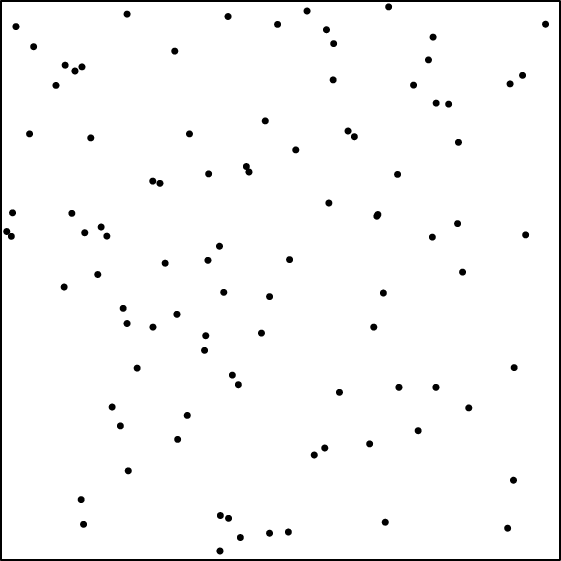
\includegraphics[width=6.5cm]{../png/ranlux1}}}
\caption{Two-dimensional vectors plotted by position in the unit square.
The {\tt ranlux} random number generator was used to produce $200$
coordinates, paired to make $100$~vectors.
\label{fig:ranlux}}
\end{figure}
\begin{figure}
\centerline{\rotatebox{270}{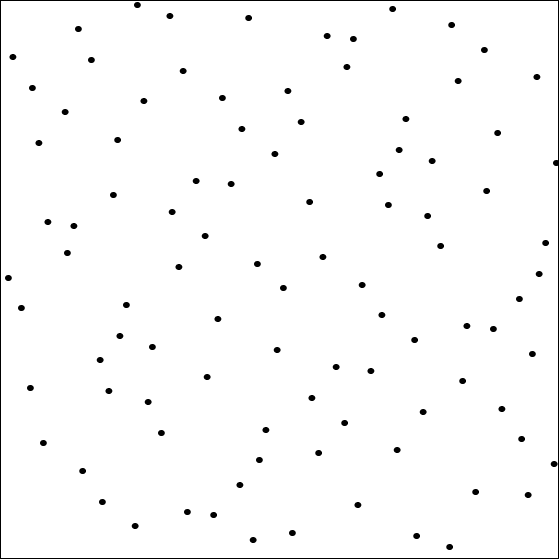
\includegraphics[width=6.5cm]{../png/halton1}}}
\caption{Two-dimensional vectors plotted by position in the unit square.
The {\tt halton} quasi-random number generator was used to produce $100$~vectors.
\label{fig:halton}}
\end{figure}

The Halton sequence is important because it can be defined without
setting a definite number of samples~$N_a$ in advance, hence it can be
used just like sequences from standard Monte-Carlo random number generators.
This contrasts with the Hammersley sequence, where the first component of
each vector is~$l/N_a$, then other components contain van der Corput sequences.
However, much of
Niederreiter's book is concerned with cases where $N_a$ is specified in advance,
when it transpires for example that $A_2$ may be reduced to as little as~$0.26$, using a $(t,s)$~sequence.

The definition of $(t,s)$~sequences is quite involved. The main idea is to
generate the quasi-random sequences as sets of vectors of dimension~$s$ 
(hence the $s$ in the name) rather than as in Halton where the components
of the vectors are computed independently as $1$-D van der Corput sequences.
The $t$ denotes the fact that, instead of each integer being represented in base~$b$
prior to bit reversal, it is represented in base~$b^{t+1}$. Hence,
in the $(t,s)$~notation,  van
der Corput sequences are $(0,1)$~sequences, and anyway apparently $t=0$
has optimally small error.
%Software for $(t,s)$~sequences
%is available from ACM~TOMS on the web~\cite{Br94Prog} and has been downloaded and tested.

Returning to Halton sequences,
the expression for discrepancy in $d$-D is
\begin{equation}
\epsilon_N = A_d (\ln N)^d/N
\end{equation} 
where the values of $A_d$ are tabulated in Niederreiter's Table~4.4.~\cite[p.96]{niederreiter}.
The first few are $A_d = 0.66, 0.82, 1.26, 2.62$, for~$d=2,3,4,5$. At higher~$d$,
$A_d$ increases rapidly so that for example, $A_{12} = 16\,800$ and
$A_{20}=6.62 \times 10^{10}$, whereas the corresponding value~$C_d$ for the
best $(t,s)$ sequence \emph{decreases} almost as rapidly ($C_6=0.0186$).
This is the benefit  gained from the greater complexity of 
calculating the $(t,s)$~sequences.

Despite the theory, much practical experience with QMC
as reported and performed by Morokoff~\emph{et al}~\cite{Mo94Quas,Mo95Quas}
suggests that QMC frequently performs little better than MC
when $d$ is large. Morokoff~\emph{et al} considered Halton sequences
and $(t,s)$ sequences in base~$b=2$ (referred to as Sobol sequences)
and in other prime number bases (Faure sequences).
It seems that for the variety of methods tested,
the number of sample points required for the asymptotic discrepancy
estimates to be realised can increase exponentially with dimension~$d$,
so the curse of dimensionality remains.
There is evidence however that in some problems, where only a relatively small
number of dimensions is apparently important, QMC performance
can be greatly improved~\cite{Ca97Valu}. One important point to make
is that Morokoff~\emph{et al} tended to explore more those QMC
rules which had the best asymptotic behaviour. Their results do not
exclude the possibility that the simpler techniques of
lattice rules, see ref~\cite[\S\,5.1]{niederreiter},
might have better behaviour in
practice, especially if the lattice basis~${\bf g}$ is well chosen.
Note that NAG uses the simple Korobov rule, in which the components of~${\bf g}$
are given as
\begin{equation}
g_k = a^{(k-1)} (\mod p)
\end{equation}
 for specially chosen real~$a>1$ and prime number~$p$.
%if Q is discontinuous or K is large


\subsection{Latin Hypercube Sampling}\label{sec:LHSamp}
%\subsection{Latin Hypercube Sampling}\label{sec:LHsamp}
One of the cheapest sampling strategies is stratified sampling.
The easiest variant to describe, viz.\ Latin hypercube~\cite{Mc79Comp}
is illustrated in \Fig{hcube},
after Steinberg as quoted in ref~\cite[\S\,4]{kaloswhitlock}.
The sample space is gridded, but now sample
points are required to lie within the grid squares, and in fact their
precise location within a square in determined randomly.
The selection of grid-square is also random, but heavily constrained
by the fact that no other sampled square should have the same
discrete co-ordinate values in any co-ordinate. For example,
in \Fig{hcube}, the fact that there is a sample point in the
square three along from the left in the bottom row, discrete
coordinate~$(3,1)$, means that no sample will be placed in
cells with coordinates~$(3,j)$ or~$(i,1)$ for any~$i$ or~$j$.
If there are~$N_1$ cells in each coordinate, the
total number of samples needed is also~$N_1$.
This is very cheap, but the method is known to
become unreliable when the parameters' variations are correlated.
\begin{figure}
\centerline{\rotatebox{0}{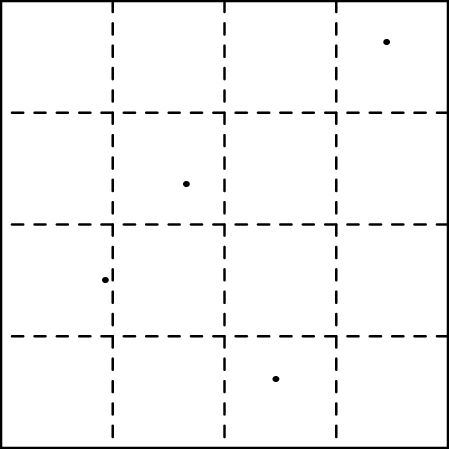
\includegraphics[width=6.5cm]{../png/hcube}}}
\caption{\label{fig:hcube}
 Latin hypercube sampling.}
\end{figure}

%\section*{References}
\bibliographystyle{unsrt}
\bibliography{../bib/new,../bib/waynes,../bib/misc,../bib/warv,../bib/neuts,../bib/reac,../bib/exc,../bib/active,../bib/dg1srt,../bib/mc}

\end{document}
